\chapter*{Uvod}
\addcontentsline{toc}{chapter}{Uvod}
\markboth{Uvod}{Uvod}

Od malih nogu društvo nas uči da je sposobnost pisanja i čitanja jako
važna pa te tehnike usvajamo brzo. Ne čini nam se da u tome postoji nešto teško.
Naprotiv, pisanje i čitanje nam izgledaju potpuno prirodno. Međutim, budući da smo ipak
naučeni pisati i da je pisanje izrazito kompleksno, s puno pravila
i još više iznimaka, često pišemo neispravno.
Tako, primjerice, griješimo
zbog nedostatne obrazovanosti (gramatičke i pravopisne pogreške)
ili pak utjecaja okruženja u kojem živimo (dijalekti). Neispravno možemo
pisati i zbog alata koje koristimo pri pisanju
(pritiskanje krive tipke na tipkovnici)
ili zbog utjecaja drugih kultura na razvoj
alata u svakodnevnom životu (mijenjanje {\glqq}č'' u {\glqq}c'' zbog jednostavnosti
zapisa u računalu). Neke od tih grešaka ne smatramo problematičnim
i učestale su u jeziku dok neke druge pak smatramo velikim greškama
jer mijenjaju semantiku napisane riječi.

Metoda uočavanja učestalih grešaka i općenito transformacija nad riječima
jako je zanimljiv aparat pri modeliranju i proučavanju
prirodnih jezika. Recimo, metoda poput one koja mjeri sličnost između napisanih
riječi ili općenitije nizova znakova.

No, nisu nužno zanimljive samo pogreške ili transformacije nad slovima
određene riječi već i strukture koje tvori više riječi poput,
primjerice, poštanskih adresa.
Također, zanimljivo je i na koje se sve načine pišu
poštanske adrese u kolokvijalnom pismu kao i kolika je
vjerojatnost da neki niz znakova tvori poštansku adresu.

Zanimljivi mogu biti i odnosi između entiteta opisani s nekim
skupom standardnih riječi poput ključnih riječi u opisima
znanstvenih članaka ili pak riječi koje služe kao poveznice
između WWW adresa na internetu.

Osim prirodnih jezika i pripadnih riječi, slova se danas koriste
i za opisivanje drugih struktura. Primjerice, DNA nizovi se standardno
prikazuju kao nizovi slova A, C, G i T. Čak se i pojam palindroma
poput {\glqq}Ana voli Milovana'' može na odgovarajući način definirati
za nizove znakova u DNA nizovima. Pogreškama u DNA nizovima
možemo smatrati mutacije. Mutacije su promjene nasljedne
informacije jednog organizma.
Uzroci mutacija su mnogobrojni: greške pri umnožavanju genetskog materijala 
u procesu stanične diobe, izlaganje vanjskim čimbenicima poput radijacije
i slično. Mutacije ne moraju nužno biti loše te se one u spolnim stanicama
smatraju jednim od preduvjeta evolucije. Time je modeliranje
pogrešaka ili transformacija nad DNA nizovima izrazito zanimljivo.

Iz rečenog nam se čini da nizovi znakova (uglavnom slova)
tvore zanimljive strukture za proučavanje.

Namjera je ovog doktorskog rada prikazati svojstva nekih od tih struktura:
palindroma u DNA nizovima, poštanskih adresa u hrvatskom jeziku,
pogrešaka ili transformacija pri pisanju riječi te
komponenata grupiranih riječima ili slovima.
Točnije, namjera je matematički modelirati strukture i
procese kod tih struktura.

Kao prvu zanimljivu strukturu u doktorskom radu proučavamo palindrome
u DNA nizovima. Palindromi su većini poznati kao nizovi slova
koji se čitaju ili izgovaraju isto od početka ili kraja. 
U DNA nizovima palindrome definiramo na sličan način kao i
u prirodnim jezicima.
Isto čitanje s oba kraja je nužno,
ali uz prethodnu operaciju komplementiranja znakova.
Recimo, za niz \nzdna{ACGT} bi definiranjem komplementarnosti
putem prirodnog uparivanja baza $A \sim T$ i $C \sim G$ definirali
komplementaran niz sa \nzdna{TGCA} te bi rekli da je početni niz
palindrom jer se čita od početka isto kao i njemu komplementarni
od kraja. Potreba za definiranjem palindroma u DNA nizovima,
i proučavanje istih, može se činit čudnom. Međutim, ako 
primijetimo da palindromi u DNA nizu opisuju spajanje između
dva dijela DNA niza onda nam motivacija postaje bliža.
Naime, ako imamo palindrom u jednoj
niti DNA niza onda se ta nit može spojiti sama sa sobom umjesto
da se poveže s drugom niti te time tvoriti strukturu ukosnice
(slika \ref{uvod:fig:ukosnice}).
Štoviše, dosadašnja su istraživanja pokazala da su palindromi
u molekuli DNA nužni za funkcioniranje genoma
(pogledati potpoglavlje
\ref{pal:sec:referencework}
za reference).

\begin{figure}
	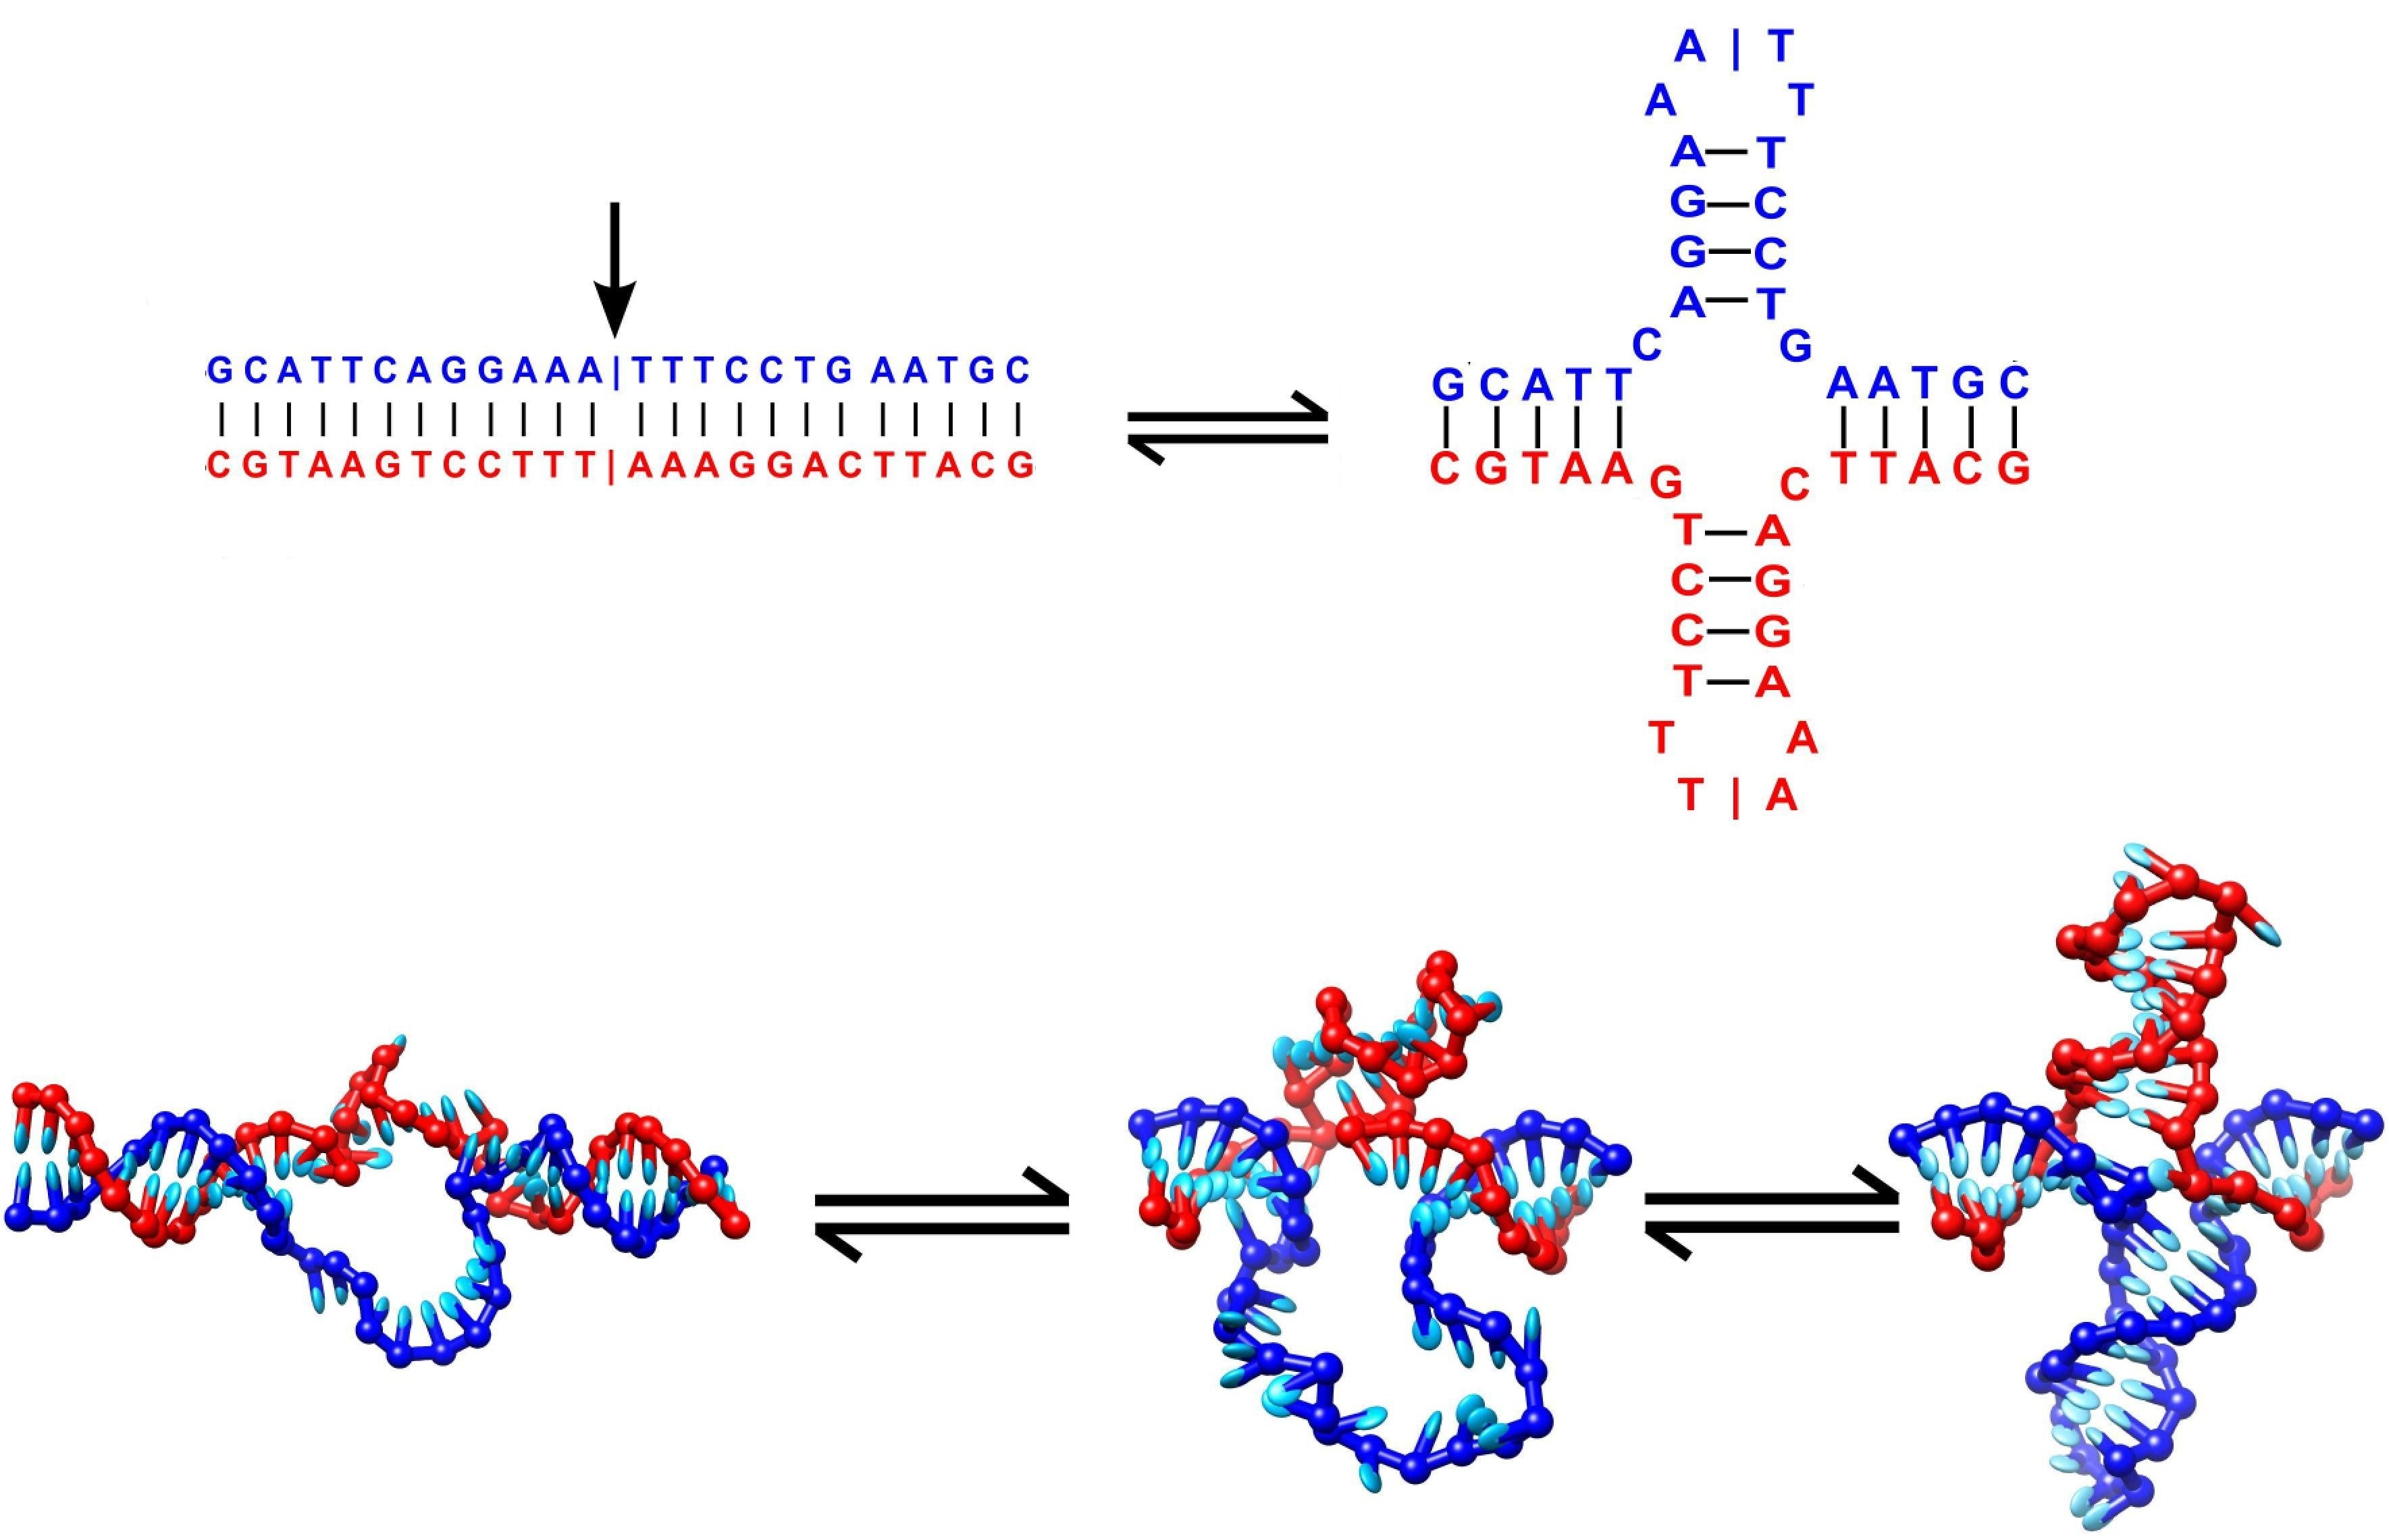
\includegraphics{./poglavlja/uvod/slike/PCA290_A.jpg}
	\caption{Stvaranja ukosnica iz palindroma u DNA nizu
		prikazano pomoću slovčanog i molekularnog
		prikaza DNA niza (izvor \cite{dna_cruciforms}).
		Strelica označava centar palindroma.}
		\label{uvod:fig:ukosnice}
\end{figure}

Budući da su palindromi značajni za funkcioniranje genoma
koristan bi bio nekakav oblik statističkog testa koji bi
odavao ima li palindroma određene duljine značajno više ili manje
od očekivanog broja unutar nekog npr. roda koji se proučava.
Iskaz rezultata koji omogućavaju konstrukciju takvog testa
bit će prezentiran u poglavlju \ref{ch:palindromi} ovog doktorskog rada.


\section*{Doprinosi doktorskog rada}
\addcontentsline{toc}{section}{Doprinosi doktorskog rada}

\begin{itemize}[label=$\bullet$]
	\item{
		Definiran je novi model nizova znakova pomoću
		blokova koji se periodično ponavljaju ili 
		zadržavaju fiksan omjer porastom duljine niza.
		Distribucije znakova unutar blokova su
		jednake, ali ne i nužno iste među blokovima.
		Iskazan je i dokazan teorem o asimptotskoj
		normalnosti broja palindroma fiksne duljine
		u takvim nizovima uz uvjet nezavisnosti.
		Dani su uvjeti na 
		odgovarajuće procjenitelje
		za primjenu na nizovima
		kod kojih treba procjeniti parametre.
	}
\end{itemize}

\section*{Pregled doktorskog rada po poglavljima}
\addcontentsline{toc}{section}{Pregled doktorskog rada po poglavljima}

Prvo poglavlje naslovljeno {\glqq}Pregled poznatih rezultata
i tehničkih metoda'' prezentira neke od najvažnijih
ideja, rezultata i tehničkih metoda koje će biti
potrebne u daljnjim poglavljima kao motivacija
ili tehnički alat. 

U drugom poglavlju  naslovljenom
{\glqq}Distribucija broja palindroma u nizovima znakova''
iskazan je i dokazan teorem o asimptotskoj normalnosti
broja palindroma u nizu znakova modeliranog blokovima.
Dopuštena su dva oblika blokova (periodično ponavljajući
te fiksnog omjera unutar niza) s proizvoljnim
distribucijama znakova unutar blokova.
Nezavisnost svih znakova se pretpostavlja.
Također, dani su uvjeti na procjenitelje za
očekivanje i varijancu pri korištenju asimptotske
normalnosti na nizove kod kojih je potrebno procjeniti
parametre modela. Iznesene su i formule 
za očekivanje i kovarijance palindroma s
proizvoljnim distribucijama. Primjerom primjene
rezultata na stvaran DNA niz prikazana je 
razlika između n.j.d modela te modela s blokovima.
Kvaliteta aproksimacije prezentirana je rezultatima
simulacijske studije.
Na kraju poglavlja dane su određene
primjedbe i zaključak.

\section*{Oznake, kratice i slično}
\addcontentsline{toc}{section}{Oznake, kratice i slično}

Pojmovi koji se prvi put spominju i od značaja su u ostatku
doktorskog rada podebljani su i u kurzivu:
\be{tenzor}, \be{procjenitelj}, \ldots.

\emph{Skalari} će se označavati malim slovima engleske ili 
grčke abecede: $a,b,c,\gamma,\ldots$.

\emph{Vektori} će se označavati malim podebljanim slovima engleske
abecede, a njihovi elementi koristit će indekse.
Na primjer, $v_i$ je $i$-ti element vektora
$\tv{v}=(v_i)_{i=1}^{n}=(v_1,\cdots,v_n)$.
U rijetkim slučajevima, zbog lakše preglednosti,
koristit će se i oznaka $v[i]$ za elemente vektora.

\emph{Matrice} će se označavati velikim slovima engleske
abecede: $\tmatrix{A},\tmatrix{B},\tmatrix{C},\ldots$.
Matrični elementi označavat će se sa
$M_{i,j}=M_{ij}$ ili s $M[i,j]$. Iznimno
će se elementi matrice označavati drukčije
(zadržavajući sintaksu i semantiku) kada
elementima definiramo matricu, npr. $M=[m_{ij}]$.
Za danu matricu $M$
$i$-ti redak će se označavati s $M_{i,:}$ ili $M[i,:]$,
a $j$-ti stupac s $M_{:,j}$ ili $M[:,j]$.


\emph{Tenzori} će se označavati velikim podebljanim slovima
engleske abecede: $\ttenzor{X}, \ttenzor{Y}, \ttenzor{Z},\ldots$.
Elementi tenzora $\ttenzor{X}$ označavat
će se sa $\ttenzor{X}(i_{1},\cdots,i_{n})$. Kada je vektor male dimenzije
ponekad će se koristiti i oznaka $\ttenzor{X}_{i,j,k}=\ttenzor{X}_{ijk}$
za elemente tenzora.

\emph{Slučajne varijable} će se označavati velikim slovima
engleske abecede: $\tsvar{X}, \tsvar{Y}, \tsvar{Z},\ldots$.
Budući da izrazi koji sadrže slučajne varijable uglavnom neće sadržavati
i matrice dvosmislenost ne bi trebala biti problem.

\emph{Slučajni vektori} će se označavati velikim podebljanim slovima
engl. abecede: $\tsvek{X}, \tsvek{Y}, \ldots$.
Budući da izrazi koji sadrže slučajne vektore  neće sadržavati
i tenzore dvosmislenost ne bi trebala biti problem.
Često će se pisati $\tsvek{X} \in K$ da bi se istaknulo
da je kodomena slučajnog vektora $\tsvek{X}$ jednaka $K$.
Da slučajan vektor $\tsvek{X}$ pripada nekoj vjerojatnosnoj
razdiobi $\eta$ označavat će se sa $\tsvek{X}\sim \eta$.
Specifično će ponekad za diskretne distribucije oznaka biti
\[
	\tsvar{X} \sim
	\begin{pmatrix}
	a_1 & a_2 & a_3 & \cdots & a_K \\
	p_{1} & p_{2} & p_{3} & \cdots & p_{K} \\
	\end{pmatrix}
\]
kada se bude htjelo naglasiti koji su mogući ishodi slučajne varijable $X$
($\vP (\tsvar{X} = a_k) = p_{k}$ za sve $k \leq K$). 


\emph{Nizovi znakova} označavat će se velikim slovima 
koristeći efekt malog verzala (engl. \textit{small-caps}). 
Tu su mala slova zamijenjena velikim slovima manje veličine,
dok su velika jednaka običnima, primjerice: \nz{Ivan Gundulić},
\nz{matrica} ili \nz{ACGTTTGCA}. Također, u određenim će se
prilikama koristiti i kurziv pri označavanju:
\nzk{Ivan Gundulić}.


\emph{Nizovi} u matematičkom smislu označavat će se zagradama
poput $(a_k)_k$ gdje će se podrazumijevati da je $k \in \setN$.
Ukoliko bude očito po kojem se indeksu niz pomiče često će se pisati
samo $(a_k)$.

